\setcounter{chapter}{7}
\chapter{Simulation Analysis}
\label{cha:simulation_analysis}
% \minitoc
% 
% 
\section{Parameter narrowing}
% 
\begin{itemize}
    \item myelin radius ->literatur
    \item micro oder macro -> simulation
    \item dn -> trel? different density?
    \item voxelsize -> simulation
    \item n filter rho -> fixed to 9 like experiment
    \item intensity ->fixed with sigma noise
    \item LAP pixel size / which density, fiber configuration, ... can be identified
\end{itemize}
% 
% \begin{figure}[!tbh]
%     \centering
%     \resizebox{.95\textwidth}{!}{
%     % \inputtikz{gfx/test.tikz}
%     }
% 	\caption{test_plot}
% 	\label{fig:test_plot}
% \end{figure}
% 

\subsection{single fiber f}
\begin{align*}
    f(\alpha, \varphi) &= f(-\alpha, \varphi + \pi)\\
    f(\alpha, \varphi) &= f(\alpha+2\pi, \varphi)  = f(\alpha, \varphi+2\pi)\\
\end{align*}
\begin{align*}
    S:(f(\alpha, \varphi)) \rightarrow (\mathbb{R}, [0, 2 \pi), [0, 1)))\\
    S(f(\alpha, \varphi)) = S(f(\alpha, \varphi - \Delta\varphi)) + \begin{pmatrix}0\\ \Delta \varphi\\ 0\end{pmatrix}\\
    S(T(f(\alpha, \varphi), \theta, \phi) = S(T(f(\alpha+, \varphi+), -\theta, -\phi)
\end{align*}
% 
\subsection{two fiber population}
\begin{align*}
    S(f_0(\alpha, \varphi), f_1(\omega, \psi)) = \\
    T(S(f_0(\alpha, \varphi), f_1(\omega, \psi)), \theta, \phi) = 
\end{align*}
% 
\begin{figure}[!t]
\centering
\def\tikzwidth{0.45*\textwidth}
\subcaptionbox{...}[.49\textwidth]{
\inputtikz{gfx/model/sphere_models_.tikz}}
\subcaptionbox{...}[.49\textwidth]{
\inputtikz{gfx/model/sphere_models.tikz}}
\caption{...}
\end{figure}
% 
\subsection{simulation sampling}
% 
\begin{itemize}
    \item \micro or \macro
    \item \voxelsize
\end{itemize}

to identify the needed optical resolution inside the simulation, the \voxelsize and \model(\micro or \macro) will be analysed.
The question is, how big can the \voxelsize be so that the resulting signal (for one \ac{PM} pixel) is not significantly different.
The same is true for the choice of \model.
The simulation setup is as follows:

\begin{table}[!b]
\centering
\pgfplotstabletypeset[
    column type=l,
    every even row/.style={before row={\rowcolor[gray]{0.95}}},
    % columns/person/.style={column name=},
    % columns/singEnglish/.style={column name=English},
    % columns/singGaeilge/.style={column name=Gaeilge},
    columns/variable/.style={string type},
    columns/value/.style={string type},
    % colums/value/.style={},
    % empty cells with={--}, % replace empty cells with '--'
    every head row/.style={before row=\toprule,after row=\midrule},
    every last row/.style={after row=\bottomrule},
    col sep=&,
    row sep=\\,
    % string type,
]
{variable & value\\
simpli.pixel\_size & \SI{1.25}{\micro\meter}\\
simpli.sensor\_gain & \SI{1.5}{}\\
simpli.optical\_sigma & \SI{0.71}{}\\
% simpli.filter\_rotations & np.linspace(0, np.pi, 9, False)\\
simpli.interpolate & \SI{1}{}\\
simpli.untilt\_sensor\_view & \SI{1}{}\\
simpli.wavelength & \SI{525}{\nano\meter}  \\
simpli.light\_intensity & \SI{50000}{\arbitraryunit} \\
% simpli.tilts & \SI{np.deg2rad(np.array([(0, 0)]))}{}\\
simpli.voxel\_size & \$\voxelsize\\
% \multirow{2}{*}{simpli.set\_voi} & $-\SIlist[list-units = brackets,list-final-separator={, },]{0.5;0.5;30}{\micro\meter}$\\
simpli.set\_voi & $-\SIlist[list-units = brackets,list-final-separator={, },]{0.5;0.5;30}{\micro\meter}$\\
& $\phantom{-}\SIlist[list-units = brackets,list-final-separator={, },]{0.5;0.5;30}{\micro\meter}$\\
}
\caption{simulation setup}
\end{table}
% 
% 
% \begin{lstfloat}[!tb]
% \lstset{
% language=python,
% keywordstyle=\color{blue},
% stringstyle=\color{red},
% commentstyle=\color{green!60!black},
% tabsize=2
% }
% \begin{lstlisting}
% PIXEL_SIZE = 1.0
% FIBER_RADII = 1.0
% THICKNESS = 60

% simpli.pixel_size = PIXEL_SIZE
% simpli.sensor_gain = 1.5  # in micro meter
% simpli.optical_sigma = 0.71  # in voxel size
% simpli.filter_rotations = np.linspace(0, np.pi, 9, False)
% simpli.interpolate = True
% simpli.untilt_sensor_view = True
% simpli.wavelength = 525  # in nm
% simpli.light_intensity = 50000  # a.u.
% simpli.tilts = np.deg2rad(np.array([(0, 0)]))
% simpli.voxel_size = voxel_size
% simpli.set_voi(-0.5 * np.array([PIXEL_SIZE, PIXEL_SIZE, THICKNESS]),
%               0.5 * np.array([PIXEL_SIZE, PIXEL_SIZE, THICKNESS]))
% simpli.dim_origin = [10, 10, -0.5 * THICKNESS]
% \end{lstlisting}
% \label{alg:voxel_size_setup}
% \caption{voxel\_size\_setup}
% \end{lstfloat}
% 
% 
% \begin{figure}[!t]
%     \resizebox{\textwidth}{!}{
%     \inputtikz{gfx/model/sphere_discretization.tikz}
%     }
% 	\caption{sphere\_discretization}
% 	\label{fig:sphere_discretization}
% \end{figure}
% % 
% \begin{figure}[!t]
%     \resizebox{\textwidth}{!}{
%     \inputtikz{data/5/voxel_size_vs_diff_dir.tikz}
%     }
% 	\caption{voxel\_size\_vs\_diff\_dir}
% 	\label{fig:voxel_size_vs_diff_dir}
% \end{figure}
% 
%  MACHT PROBLEME FIXME:
% \begin{figure}[!t]
%     \resizebox{\textwidth}{!}{
%     \inputtikz{data/5/voxel_size_vs_retardation.tikz}
%     }
% 	\caption{voxel\_size\_vs\_retardation}
% 	\label{fig:voxel_size_vs_retardation}
% \end{figure}
% 
% \begin{figure}[!t]
% \resizebox{\textwidth}{!}{
% 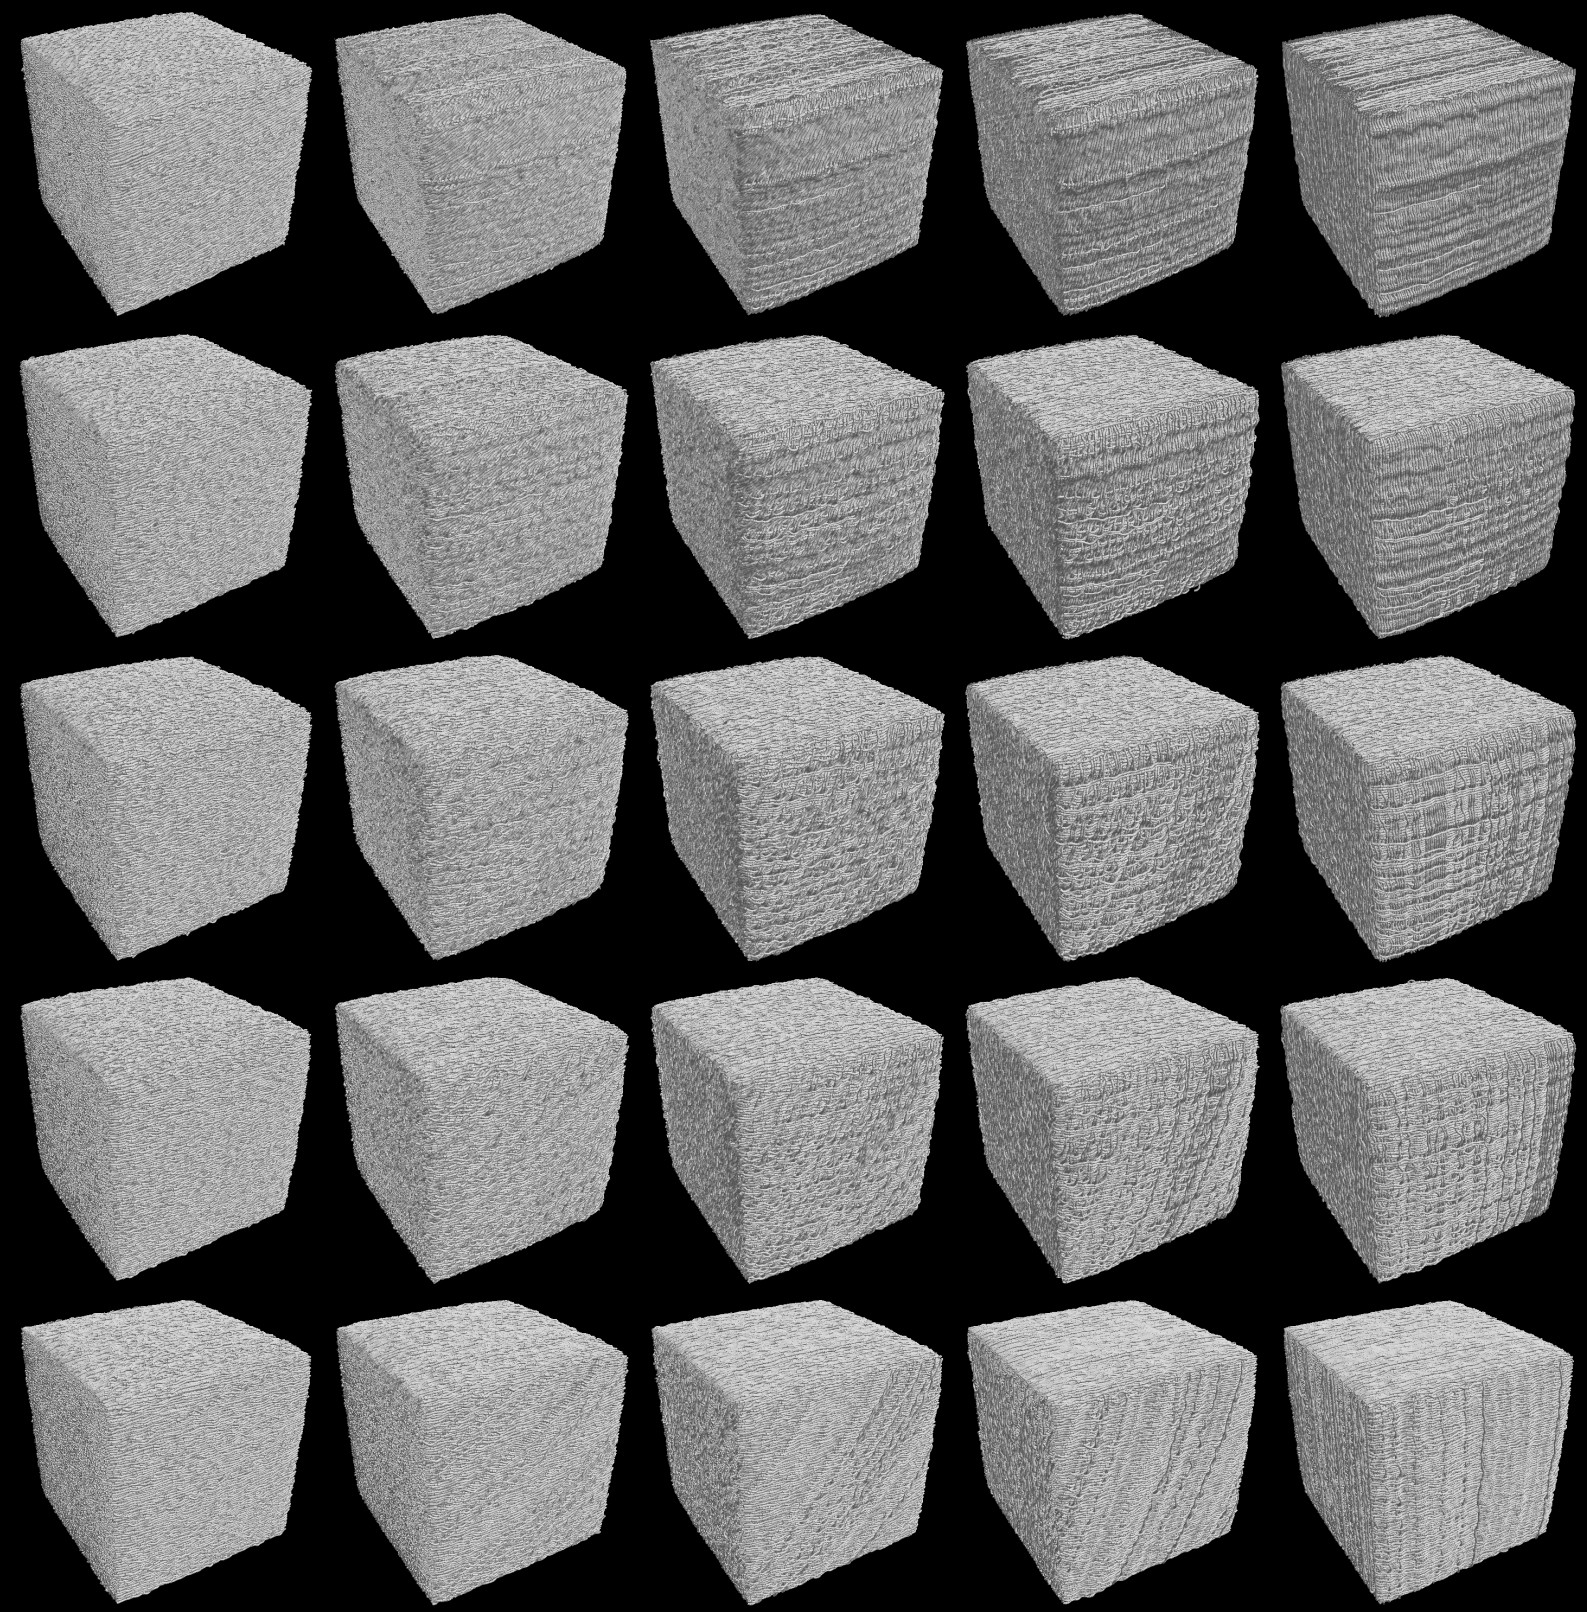
\includegraphics[]{gfx/model/cube_2pop_montage.jpg}
% %\begin{minipage}{30cm}
% %%\foreach \psi [count=\i] in {0.1, 0.2, 0.3, 0.4, 0.5, 0.6, 0.7, 0.8, 0.9}{
% %%	\foreach \omega in {0.0, 10.0, 20.0, 30.0, 40.0, 50.0, 60.0, 70.0, 80.0, 90.0}{	
% %\foreach \psi [count=\i] in {0.1, 0.3, 0.5, 0.7, 0.9}{
% %    \foreach \omega in {10.0, 30.0, 50.0, 70.0, 90.0}{
% %        \includegraphics[trim={110, 70, 90, 130}, clip, width=6cm] %width=2.5cm
% %        {dev/data/cube_2pop/cube_2pop_psi_\psi_omega_\omega_.solved.ppm.png}
% %        \hspace{-0.5cm}
% %    }
% %    \vspace{-0.1cm}
% %    \ifthenelse{\i<9}{\newline}{}
% %}
% %\end{minipage}
% }
% \caption{A test}
% \end{figure}
% 
% 
% 
% TODO:
% \begin{figure}[!t]
% \resizebox{\textwidth}{!}{
% \foreach \omega in {0,30,60,90} {
%     \resizebox{0.215\textwidth}{!}{
%     \input{dev/data/pm_omega_\omega.0_psi_epa_dir.tikz}
%     }
% }}
% \resizebox{\textwidth}{!}{
% \foreach \omega in {0,30,60,90} {
%     \resizebox{0.215\textwidth}{!}{
%     \input{dev/data/pm_omega_\omega.0_psi_epa_ret.tikz}
%     }
% }}
% \caption{A test}
% \end{figure}

% 
\section{Optimal Grid Size}

\subsection{Impact on labelfield}
% 
\tikzexternaldisable
% 
\begin{figure}[!t]
\centering
\resizebox{1.0\textwidth}{!}{
\inputtikz{gfx/simpli/vector_error.tikz}}
\caption[Discretization error]{Discretization error.
This behavior is much stronger with myelin layers}
\label{fig:vectorfield_disc_error}
\end{figure}
% 
\tikzexternalenable
% 
\subsection{Impact on vektorfield}
% 
slerp and multisampling and sparse vectorfield
% 
\begin{figure}[!t]
\centering
\resizebox{0.95\textwidth}{!}{
\subcaptionbox{yz-view}[.3\textwidth]{
\includegraphics[width=0.3\textwidth,page=1]{dev/gfx/1/vector_field_0.2.pdf}}
\subcaptionbox{zx-view}[.3\textwidth]{
\includegraphics[width=0.3\textwidth,page=2]{dev/gfx/1/vector_field_0.2.pdf}}
\subcaptionbox{xy-view}[.3\textwidth]{
\includegraphics[width=0.3\textwidth,page=3]{dev/gfx/1/vector_field_0.2.pdf}}
}
\caption{Discretization}
% \label{fig:vd1}
\end{figure}

\begin{figure}[!t]
\centering
\resizebox{0.95\textwidth}{!}{
\inputtikz{dev/gfx/1/vector_field_mode_plot_0.20_5_r.tikz}
}
\caption{NN, Lerp, Slerp}
% \label{fig:vd1}
\end{figure}
% 
% \subcaptionbox{}[.245\textwidth]{
% \begin{figure}[!t]
% \centering
% \resizebox{0.75\textwidth}{!}{
% \inputtikz{dev/gfx/1/optical_axis_high_norm_1.00_19.0_r.tex}}
% \caption{Discretization error}
% \label{fig:vd1}
% \end{figure}
% % 
% \begin{figure}[!t]
% \centering
% \resizebox{0.75\textwidth}{!}{
% \inputtikz{dev/gfx/1/optical_axis_high_norm_0.50_9.0_r.tex}}
% \caption{Discretization error}
% \label{fig:vd2}
% \end{figure}
% % 
% \begin{figure}[!t]
% \centering
% \resizebox{0.75\textwidth}{!}{
% \inputtikz{dev/gfx/1/optical_axis_high_norm_0.20_4.0_r.tex}}
% \caption{Discretization error}
% \label{fig:vd3}
% \end{figure}
% 
\paragraph{Macro}
\paragraph{Micro}
% 
\subsection{Impact on data}
%
\begin{figure}[!t]
\centering
\resizebox{0.75\textwidth}{!}{
\inputpdf{dev/gfx/5/foo_p_zoom.pdf}}
\caption{}
\label{fig:foo_p_zoom}
\end{figure}
% 
\begin{figure}[!t]
\centering
\resizebox{0.75\textwidth}{!}{
\inputpdf{dev/gfx/5/foo_r.pdf}}
\caption{}
\label{fig:foo_r}
\end{figure}
% 
\begin{figure}[!t]
\centering
\resizebox{0.75\textwidth}{!}{
\inputpdf{dev/gfx/5/foo_r_zoom.pdf}}
\caption{}
\label{fig:foo_r_zoom}
\end{figure}
% 
\begin{figure}[!t]
\centering
\resizebox{0.75\textwidth}{!}{
\inputpdf{dev/gfx/5/foo_p_noise.pdf}}
\caption{}
\label{fig:foo_p_noise}
\end{figure}
% 
\begin{figure}[!t]
\centering
\resizebox{0.75\textwidth}{!}{
\inputpdf{dev/gfx/5/foo_r_noise.pdf}}
\caption{}
\label{fig:foo_r_noise}
\end{figure}
% 
\paragraph{Macro}
\paragraph{Micro}
% 
\subsection{Impact on modalities}
\paragraph{Macro}
\paragraph{Micro}
% 
\section{LAP PM impact}
\paragraph{LAP}
können vereinfachte modelle genutzt werden?, p-doppelbrechnung, gröser radius, ...
\paragraph{PM}
% 
\section{CPU Acceleration}
% 
acceleration of individual compontes, e.g. generation, simulation, apply optics, rofl, ...
